% Licensed to the Apache Software Foundation (ASF) under one or more
% contributor license agreements. See the NOTICE file distributed with
% this work for additional information regarding copyright ownership.
% The ASF licenses this file to You under the Apache License, Version 2.0
% (the ``License''); you may not use this file except in compliance with
% the License. You may obtain a copy of the License at
%
% http://www.apache.org/licenses/LICENSE-2.0
%
% Unless required by applicable law or agreed to in writing, software
% distributed under the License is distributed on an ``AS IS'' BASIS,
% WITHOUT WARRANTIES OR CONDITIONS OF ANY KIND, either express or implied.
% See the License for the specific language governing permissions and
% limitations under the License.

\subsubsection{Configuring a Documentum Repository}

You must fill in the following extra fields if you choose to
configure a Documentum repository connection: 

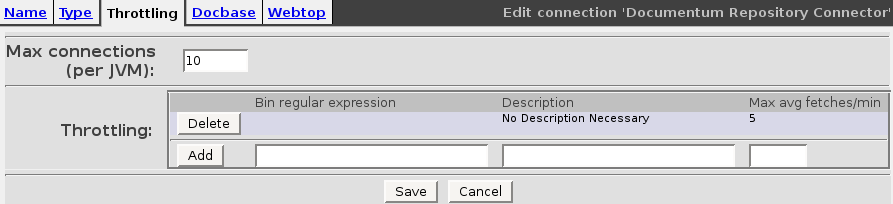
\includegraphics[width=300pt]{Docu-edit-repository-tab3}


\begin{itemize}

\item \textbf{Max connections (per JVM):} \ifCombinedConnectorGuide \label{maxrepocon} \fi Here you can set the maximum
number of connections to your repository.

The maximum number of connections per JVM is important for three
reasons.  First, the number of connections may impact the licensing on
your document server, depending on the repository. If you have a
finite number of Documentum connections available, they will be split
between the authority connector, which authorizes user access to
documents, and the repository connector, which actually downloads the
documents to the appliance. As in the case of the authority
connection, the default value of 10 connections may be a larger
portion of the available connections than you would like the GTS
appliance to use.

Second, the number of connections may impact the resources
available on the appliance. If the connector framework is slowing down
your appliance, lowering this number should help.

Third, only ten document streams can be processed by the appliance at
one time.  If you are also using other repository connectors or the
\command{ingest} command on the appliance, you should reduce this
number to prevent contention for the Ingestion interface. The
Documentum Connector will never overwhelm the interface on its own,
but when other applications are also using the ingestion interface, it
may be best to set the number of repository connections to five or
even fewer.

\item \textbf{Throttling:} Throttling allows you to limit the rate of
document ingestion based on document bins that you create with regular
expressions.

The maximum fetch rate allows you to set three things: Expression,
description, and fetches per minute. Expression allows you to provide
a regular expression to match against document bins. Each document
ingested through a connector is associated with one or more document
bins. These bins represent the servers that the connector interacts
with to obtain the document. Typically, a document will be associated
with only one document bin, representing the repository server hosting
the document. For some repository connections, documents ingested
through the connector can be hosted by different servers. In the
Documentum Connector, documents can only come from one docbase, which
you will set on the following tab. Simply leave the expression blank;
this will match any docbase you enter on the following tab.  All you
need to set is the number of document fetches per minute.  Description
is an optional field that allows you to provide a short text
description of the throttle.  Once you have set the fetch rate and
optional description, click Add.

\end{itemize}

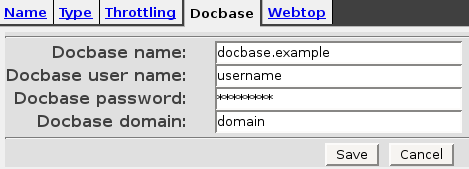
\includegraphics[width=300pt]{Docu-edit-repository-tab4}

\begin{itemize}

\item \textbf{Docbase name:} The host name of the Documentum
repository (or ``docbase'') with which you wish to connect.

\item \textbf{Docbase user name:} The user name that the GTS appliance
will use to connect to the docbase for this repository connection.
Typically, your Documentum administrator will create this account
specifically for use by the appliance. The account used by the GTS
appliance must have sufficient authority to retrieve files and their
corresponding ACLs. This may or may not be the same account used by
the GTS appliance for authority connections, depending on the security
model enforced by your Documentum administrator.

\item \textbf{Docbase password:} The password corresponding to the
username given to the GTS.

\item \textbf{Docbase domain:} The domain that the docbase is part of,
typically an Active Directory domain. This is an optional argument.

\end{itemize}

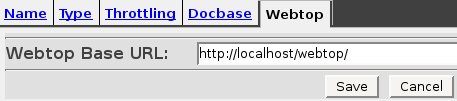
\includegraphics[width=300pt]{Docu-edit-repository-tab5}

\begin{itemize}

\item \textbf{Webtop Base URL:} The URL of the Webtop server that the
GTS appliance will use to provide MetaCarta Web Search Interface users
with document links in search results. It is recommended that you
select a Webtop server that connects to the same docbroker that the
GTS appliance uses.

\end{itemize}

After entering this information, you will be taken to the status page
for this repository connection:

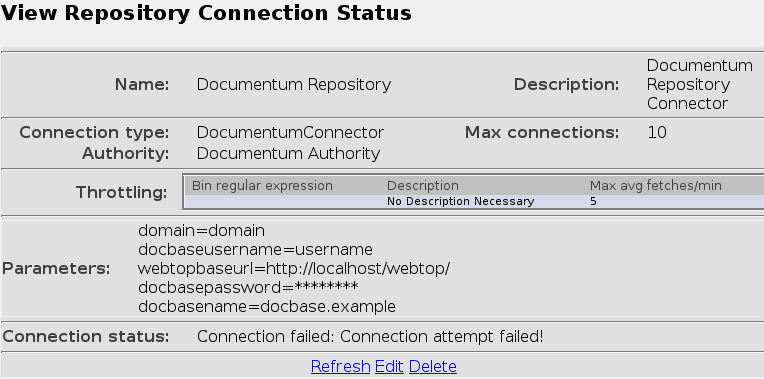
\includegraphics[width=300pt]{Docu-view-repo-conn-status}

In this example (which does not contain accurate information for any
Documentum server), the Connection Status is ``Connection failed.''
If you see this message, you most likely have incorrectly entered one
of the fields, and should click ``Edit'' to fix the data. If you have
entered everything as you intended, please inform your Documentum
administrator; you may not have been given the correct information.

